\begin{center}
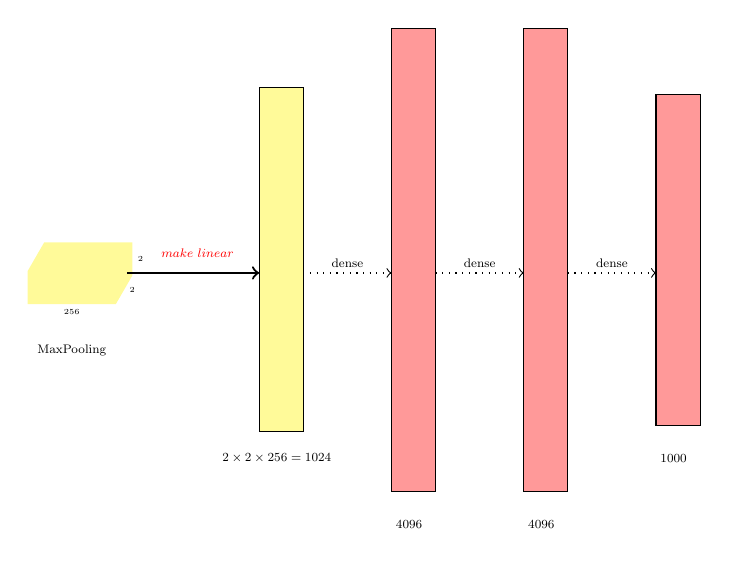
\begin{tikzpicture}[scale=0.56,transform shape]

\pgfsetxvec{\pgfpoint{2cm}{0cm}}
\pgfsetyvec{\pgfpoint{0cm}{1.5cm}}
\pgfsetzvec{\pgfpoint{-.5*1.5cm}{-.866*1.5cm}}

\def\cuboid#1#2#3#4#5{
\begin{scope}
\edef\mycolor{#2}
\edef\depth{#3}
\edef\height{#4}
\edef\width{#5}
\draw[black,fill=\mycolor, fill opacity=0.4, text opacity=1] #1 -- ++(-\depth,0,0) -- ++(0,-\height,0) -- ++(\depth,0,0) -- cycle #1 -- ++(0,0,-\width) -- ++(0,-\height,0) -- ++(0,0,\width) -- cycle  #1 -- ++(-\depth,0,0) -- ++(0,0,-\width) -- ++(\depth,0,0) -- cycle;
\end{scope}
}

\def\cuboidlabel#1#2#3#4#5#6#7#8{
\begin{scope}
\edef\mycolor{#2}
\edef\depth{#3}
\edef\height{#4}
\edef\width{#5}
\edef\depthlabel{#6}
\edef\heightlabel{#7}
\edef\widthlabel{#8}
\draw[draw=none,fill=\mycolor, fill opacity=0.4, text opacity=1] #1 -- ++(-\depth,0,0) -- ++(0,-\height,0) -- ++(\depth,0,0) node[black,pos=0.5,below] {\tiny \depthlabel} -- cycle #1 -- ++(0,0,-\width) -- ++(0,-\height,0) node[black,pos=0.5,right] {\tiny \heightlabel} -- ++(0,0,\width)  node[black,pos=0.5,below,right] {\tiny \widthlabel} -- cycle  #1 -- ++(-\depth,0,0) -- ++(0,0,-\width) -- ++(\depth,0,0) -- cycle;
\end{scope}
}

\def\kernel#1#2#3#4#5#6{
\begin{scope}
\edef\mycolor{#2}
\edef\depth{#3}
\edef\height{#4}
\edef\width{#5}
\draw[black,fill=\mycolor, fill opacity=0.4, text opacity=1] #1 -- ++(-\depth,0,0) -- ++(0,-\height,0) -- ++(\depth,0,0) -- cycle #1 -- ++(0,0,-\width) -- ++(0,-\height,0) -- ++(0,0,\width) -- cycle  #1 -- ++(-\depth,0,0) -- ++(0,0,-\width) -- ++(\depth,0,0) -- cycle;

\draw[dotted] #1 -- #6 #1++(0,0,-\width) -- #6 #1++(0,-\height,0) -- #6 #1++(0,-\height,-\width) -- #6;

\end{scope}
}

\def\kernellabel#1#2#3#4#5#6#7#8#9{
%#6 is target pixel
\begin{scope}
\edef\mycolor{#2}
\edef\depth{#3}
\edef\height{#4}
\edef\width{#5}
\edef\depthlabel{#7}
\edef\heightlabel{#8}
\edef\widthlabel{#9}
\draw[draw=none,fill=\mycolor, fill opacity=0.4, text opacity=1] #1 -- ++(-\depth,0,0) -- ++(0,-\height,0) -- ++(\depth,0,0) -- cycle #1 -- ++(0,0,-\width) -- ++(0,-\height,0) node[pos=0.5,left] {\tiny \heightlabel} -- ++(0,0,\width)  node[pos=0.6,above] {\tiny \widthlabel} -- cycle  #1 -- ++(-\depth,0,0) -- ++(0,0,-\width) -- ++(\depth,0,0) -- cycle;

\draw[dotted] #1 -- #6 #1++(0,0,-\width) -- #6 #1++(0,-\height,0) -- #6 #1++(0,-\height,-\width) -- #6;

\end{scope}
}

%\cuboid{(24,7,0)}{white}{7}{3}{0}{256}{2}{2}

%alexnet

\onslide<1->{
\cuboidlabel{(14.5,-5,-5)}{yellow}{1}{0.5}{0.5}{256}{2}{2}
\node (a) at (14.5-0.5,-5-0.5-0.7,-5) {\footnotesize MaxPooling};
}

\onslide<2->{
\draw[thick,->] (16.5,-0.7,0) -- (18,-0.7,0);
\node (a) at (17.3,-0.4,0) {\footnotesize \color{red}{$make\ linear$}};
\cuboid{(18.5,2.1,0)}{yellow}{0.5}{5.2}{0}{256}{2}{2}
\node (a) at (18.2,-3.5,0) {\footnotesize $2\times 2\times 256 = 1024$};
}

\onslide<3->{
\draw[dotted,->] (18.5,-0.7,0) -- (19+0.5,-0.7,0) node[pos=0.5,above] {\footnotesize dense};
\cuboid{(19.5+0.5,3,0)}{red}{0.5}{7}{0}{256}{2}{2}
\node (a) at (19.2+0.5,-4.5,0) {\footnotesize 4096};
}


\onslide<4->{
\draw[dotted,->] (19.5+0.5,-0.7,0) -- (20+1,-0.7,0) node[pos=0.5,above] {\footnotesize dense};
\cuboid{(20.5+1,3,0)}{red}{0.5}{7}{0}{256}{2}{2}
\node (a) at (20.2+1,-4.5,0) {\footnotesize 4096};
}

\onslide<5->{
\draw[dotted,->] (20.5+1,-0.7,0) -- (21.5+1,-0.7,0) node[pos=0.5,above] {\footnotesize dense};
\cuboid{(22+1,2,0)}{red}{0.5}{5}{0}{256}{2}{2}
\node (a) at (21.7+1,-3.5,0) {\footnotesize 1000};
}


\end{tikzpicture}
\end{center}

